
\documentclass[nooutcomes]{ximera}
%\documentclass[space,handout,nooutcomes]{ximera}

% For preamble materials

\graphicspath{
  {./}
  {algorithms/}
  {../algorithms/}
}


%%% This set of code is all of our user defined commands
\newcommand{\bysame}{\mbox{\rule{3em}{.4pt}}\,}
\newcommand{\N}{\mathbb N}
\newcommand{\C}{\mathbb C}
\newcommand{\W}{\mathbb W}
\newcommand{\Z}{\mathbb Z}
\newcommand{\Q}{\mathbb Q}
\newcommand{\R}{\mathbb R}
\newcommand{\A}{\mathbb A}
\newcommand{\D}{\mathcal D}
\newcommand{\F}{\mathcal F}
\newcommand{\ph}{\varphi}
\newcommand{\ep}{\varepsilon}
\newcommand{\aph}{\alpha}
\newcommand{\QM}{\begin{center}{\huge\textbf{?}}\end{center}}

\renewcommand{\le}{\leqslant}
\renewcommand{\ge}{\geqslant}
\renewcommand{\a}{\wedge}
\renewcommand{\v}{\vee}
\renewcommand{\l}{\ell}
\newcommand{\mat}{\mathsf}
\renewcommand{\vec}{\mathbf}
\renewcommand{\subset}{\subseteq}
\renewcommand{\supset}{\supseteq}
\renewcommand{\emptyset}{\varnothing}
\newcommand{\xto}{\xrightarrow}
\renewcommand{\qedsymbol}{$\blacksquare$}
\newcommand{\bibname}{References and Further Reading}
\renewcommand{\bar}{\protect\overline}
\renewcommand{\hat}{\protect\widehat}
\renewcommand{\tilde}{\widetilde}
\newcommand{\tri}{\triangle}
\newcommand{\minipad}{\vspace{1ex}}
\newcommand{\leftexp}[2]{{\vphantom{#2}}^{#1}{#2}}

%% More user defined commands
\renewcommand{\epsilon}{\varepsilon}
\renewcommand{\theta}{\vartheta} %% only for kmath
\renewcommand{\l}{\ell}
\renewcommand{\d}{\, d}
\newcommand{\ddx}{\frac{d}{dx}}
\newcommand{\dydx}{\frac{dy}{dx}}


\usepackage{bigstrut}


\newenvironment{sectionOutcomes}{}{}

\usepackage{array}
%\setlength{\extrarowheight}{-.2cm}   % Commented out by Findell to fix table headings.  Was this for typesetting division?  
\newdimen\digitwidth
\settowidth\digitwidth{9}
\def~{\hspace{\digitwidth}}
\def\divrule#1#2{
\noalign{\moveright#1\digitwidth
\vbox{\hrule width#2\digitwidth}}}


\title{Decimals}
\author{Bart Snapp and Brad Findell and Jenny Sheldon}
\begin{document}
\begin{abstract}
Problems about decimal numbers.
\end{abstract}
\maketitle


%\begin{problem}
%Problem
%\begin{freeResponse}
%\begin{hint}
%Hint
%\end{hint}
%\end{freeResponse}
%\end{problem} 


\begin{problem}
On the number line below, a point is marked $A$.  Select all options which could be candidates for the value of $A$.
\begin{center}
	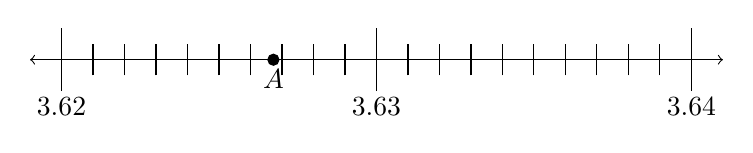
\begin{tikzpicture}[scale=2]
		\draw[<->] (-0.2,0) -- (4.2,0);
		\foreach \x in {0.2, 0.4,...,1.8, 2.2, 2.4,...,3.8} \draw (\x, -0.1)--(\x, 0.1);
		\draw (0, -0.2)--(0, 0.2);
		\draw (2, -0.2)--(2, 0.2);
		\draw (4, -0.2)--(4, 0.2);
		\node at (0, -0.3) {$3.62$};
		\node at (2, -0.3) {$3.63$};
		\node at (4, -0.3) {$3.64$};
		\draw[fill=black] (1.3456, 0) circle (1pt) node[below] {$A$};
	\end{tikzpicture}
\end{center}

\begin{selectAll}
	\choice[correct]{$3.62678$}
	\choice[correct]{$3.6267783$}
	\choice{$3.68$}
	\choice[correct]{$3.626788983$}
	\choice{$3.627$}
\end{selectAll}
\end{problem}


\begin{problem}
Select all fractions below that have terminating decimal representation.
\begin{selectAll}
	\choice[correct]{$\frac{1}{10}$}
	\choice{$\frac{1}{30}$}
	\choice[correct]{$\frac{1}{80}$}
	\choice[correct]{$\frac{1}{64}$}
	\choice[correct]{$\frac{1}{125}$}
	\choice[correct]{$\frac{1}{250}$}
	\choice{$\frac{1}{385}$}
	\choice[correct]{$\frac{1}{2048}$}
	\choice{$\frac{1}{4228}$}
	\choice[correct]{$\frac{1}{2^{19} \times 5^{47}}$}
\end{selectAll}
\end{problem}



\begin{problem}
A harder version of the previous problem: select all fractions below that have terminating decimal representation.
\begin{selectAll}
	\choice[correct]{$\frac{14}{10}$}
	\choice[correct]{$\frac{6}{30}$}
	\choice{$\frac{4}{60}$}
	\choice{$\frac{7}{98}$}
	\choice[correct]{$\frac{11}{125}$}
	\choice[correct]{$\frac{3}{150}$}
	\choice{$\frac{11}{385}$}
	\choice{$\frac{2}{2049}$}
	\choice[correct]{$\frac{1057}{4228}$}
	\choice[correct]{$\frac{3^4 \times 7^{11} \times 19}{3^2 \times 5^{22} \times 19}$}
\end{selectAll}
\begin{hint}
Don't forget to reduce the fractions to lowest terms!
\end{hint}
\end{problem}



\begin{problem}
Give an example of an irrational number.  For a challenge, don't pick $\pi$, $e$, or $\sqrt{p}$ where $p$ is prime.

\begin{freeResponse}
\begin{hint}
One of my favorites is $0.01001000100001000001\dots$.  This number's decimal representation is neither terminating nor repeating, though it {\em does} have a pattern!
\end{hint}
\end{freeResponse}

\end{problem}



\begin{problem}
Without doing the long division, after how many places would you expect $\frac{1}{47}$ to repeat?

\begin{prompt}
We expect the repetition to occur after at most $\answer[given]{46}$ places.
\end{prompt}
\end{problem}


\begin{problem}
Without doing the long division, after how many places would you expect $\frac{3}{104}$ to repeat?

\begin{prompt}
We expect the repetition to occur after at most $\answer[given]{103}$ places.
\end{prompt}
\end{problem}


\begin{problem}
Write each of the following decimals as a fraction using the patterns we observed in class.

\begin{enumerate}
	\item $0.\overline{4}$ \begin{prompt} =$\frac{\answer{4}}{\answer{9}}$ \end{prompt}
	\item $0.\overline{42}$ \begin{prompt} =$\frac{\answer{42}}{\answer{99}}$ \end{prompt}
	\item $0.\overline{215}$ \begin{prompt} =$\frac{\answer{215}}{\answer{999}}$ \end{prompt}
	\item $0.\overline{234584}$ \begin{prompt} =$\frac{\answer{234584}}{\answer{999999}}$ \end{prompt}
\end{enumerate}
\end{problem}





\begin{problem}
 It is true that $0.\overline{9} = 1$.  What do you expect the following to be equal to?
 
 \begin{enumerate}
 	\item $1.\overline{9} = \answer{2}$
	\item $0.5\overline{9} = \answer{0.6}$
	\item $2.34\overline{9} = \answer{2.35}$
	%\item $0.87893\overline{9} = \answer{0.87894}$
 \end{enumerate}
\end{problem}



\begin{problem}
Given a prime number $p$, we will explore a relationship between the number of decimal places in which $\frac{1}{p}$ repeats, and the smallest value of $n$ where $p$ divides $10^n - 1$.

Consider the case of $p=3$.  We know that $\frac{1}{3} = 0.\overline{\answer[given]{3}}$, or $\frac{1}{3}$ repeats after $\answer[given]{1}$ decimal place.  What is the smallest value of $n$ so that $3 \vert 10^n - 1$?
\begin{hint}
Choose potential values for $n$ in an organized fashion.  What is the prime factorization of $10^n-1$?
\end{hint}


\begin{prompt}
For $p=3$, we have $n=\answer{1}$.
\end{prompt}

\begin{problem}
Consider the case of $p=7$.  We know that $\frac{1}{7} = 0.\overline{\answer[given]{142857}}$, or $\frac{1}{7}$ repeats after $\answer[given]{6}$ places.  What is the smallest value of $n$ so that $7 \vert 10^n -1$?

\begin{prompt}
For $p=7$, we have $n=\answer{6}$.
\end{prompt}


\begin{problem}
Consider the case of $p=11$.  We know that $\frac{1}{11} = 0.\overline{\answer[given]{09}}$, or $\frac{1}{11}$ repeats after $\answer[given]{2}$ places.  What is the smallest value of $n$ so that $11 \vert 10^n -1$?

\begin{prompt}
For $p=11$, we have $n=\answer{2}$.
\end{prompt}

Consider the case of $p=13$.  We know that $\frac{1}{13} = 0.\overline{\answer[given]{076923}}$, or $\frac{1}{13}$ repeats after $\answer[given]{6}$ places.  What is the smallest value of $n$ so that $13 \vert 10^n -1$?

\begin{prompt}
For $p=13$, we have $n=\answer{6}$.
\end{prompt}

Consider the case of $p=37$.  We know that $\frac{1}{37} = 0.\overline{\answer[given]{027}}$, or $\frac{1}{37}$ repeats after $\answer[given]{3}$ places.  What is the smallest value of $n$ so that $37 \vert 10^n -1$?

\begin{prompt}
For $p=37$, we have $n=\answer{3}$.
\end{prompt}

What pattern are you observing?
\begin{freeResponse}
\begin{hint}
The number of places in the decimal's repeat is the same as the value of $n$.
\end{hint}
\end{freeResponse}
\end{problem}



\end{problem}



\end{problem}



\end{document}



